\label{cutflows-tables}

In this section is a breakdown of the yields at the different steps in the analysis event selection (a \textit{cutflow}) for data and important Monte Carlo simulation samples.

Data (2016-18, 126.1 \ifb):

\begin{itemize}
	\item Table \ref{tab:data_ggF_chan_4tag_cutflow}: 4b events in the ggF channel.
	\item Table \ref{tab:data_ggF_chan_2tag_cutflow}: 2b events in the ggF channel.
	\item Table \ref{tab:data_VBF_chan_4tag_cutflow}: 4b events in the VBF channel.
	\item Table \ref{tab:data_VBF_chan_2tag_cutflow}: 2b events in the VBF channel.
\end{itemize}

ggF \HH MC simulation (normalized to 126.1 \ifb):
\begin{itemize}
	\item Tables \ref{tab:mc_ggF_sm_ggF_chan_4tag_cutflow}: 4b events in the ggF channel for SM ggF \HH signal.
	\item Tables \ref{tab:mc_ggF_k10_ggF_chan_4tag_cutflow}: 4b events in the ggF channel for $\kappa_{\lambda} = 10$ ggF \HH signal.
	\item Tables \ref{tab:mc_ggF_sm_VBF_chan_4tag_cutflow}: 4b events in the VBF channel for SM ggF \HH signal.
	\item Tables \ref{tab:mc_ggF_k10_VBF_chan_4tag_cutflow}: 4b events in the VBF channel for $\kappa_{\lambda} = 10$ ggF \HH signal.
\end{itemize}

VBF \HH MC simulation (normalized to 126.1 \ifb):

\begin{itemize}
	\item Tables \ref{tab:mc_VBF_sm_VBF_chan_4tag_cutflow}: 4b events in the VBF channel for SM VBF \HH signal.
	\item Tables \ref{tab:mc_VBF_k10_VBF_chan_4tag_cutflow}: 4b events in the VBF channel for $\kappa_{\lambda} = 10$ VBF \HH signal.
	\item Tables \ref{tab:mc_VBF_k2v0_VBF_chan_4tag_cutflow}: 4b events in the VBF channel for $\kappa_{2V} = 0$ VBF \HH signal.
	\item Tables \ref{tab:mc_VBF_sm_ggF_chan_4tag_cutflow}: 4b events in the ggF channel for SM VBF \HH signal.
	\item Tables \ref{tab:mc_VBF_k10_ggF_chan_4tag_cutflow}: 4b events in the ggF channel for $\kappa_{\lambda} = 10$ VBF \HH signal.
	\item Tables \ref{tab:mc_VBF_k2v0_ggF_chan_4tag_cutflow}: 4b events in the ggF channel for $\kappa_{2V} = 0$ VBF \HH signal.
\end{itemize}

\ttbar MC simulation (normalized to 126.1 \ifb):

\begin{itemize}
	\item Table \ref{tab:ttbar_mc_ttbar_nonallhad_ggF_chan_4tag_cutflow}: 4b events in the ggF channel in \ttbar MC simulation for the non-all hadronic decay mode.
	\item Table \ref{tab:ttbar_mc_ttbar_allhad_ggF_chan_4tag_cutflow}: 4b events in the ggF channel in \ttbar MC simulation for the all hadronic decay mode.
	\item Table \ref{tab:ttbar_mc_ttbar_nonallhad_VBF_chan_4tag_cutflow}: 4b events in the VBF channel in \ttbar MC simulation for the non-all hadronic decay mode.
	\item Table \ref{tab:ttbar_mc_ttbar_allhad_VBF_chan_4tag_cutflow}: 4b events in the VBF channel in \ttbar MC simulation for the all hadronic decay mode.
\end{itemize}

% Tables:
\def\tablesversion{V2}
%data
\begin{table}
\centering
\caption{2016-18 data yields at each step in the analysis event selection for 2b and 4b events in the ggF channel, alongside the ratio of each yield to the initial yield and to the yield for the previous cut. [FEB22-unblind production (For data, expect no changes wrt MAR22)]}
\subfloat[4b data (ggF channel)]{
\centering
\label{tab:data_ggF_chan_4tag_cutflow}
\begin{tabular}{lccc}
\toprule
{} &     Yield &  Yield / Pre-selection &  Yield / Prior cut \\
\midrule
Initial (Unweighted for MC)            &  1.59e+10 &                      - &                  - \\
Pass NTuple Preselection               & 5.697e+08 &                      1 &                  - \\
Trigger                                & 2.807e+08 &                 0.4927 &             0.4927 \\
Trigger Buckets                        &  2.49e+08 &                 0.4371 &             0.8873 \\
ggF channel                            & 2.457e+08 &                 0.4314 &             0.9868 \\
$\ge$ 4 central jets, $\ge$ 2 $b$-tags & 1.806e+08 &                  0.317 &             0.7349 \\
$\ge$ 4 $b$-tags                       & 1.886e+06 &               0.003311 &            0.01045 \\
$|\Delta\eta_{hh}| < 1.5$              & 1.032e+06 &               0.001811 &             0.5469 \\
Top Veto                               & 7.506e+05 &               0.001318 &             0.7276 \\
Signal Region                          & 1.617e+04 &              2.839e-05 &            0.02154 \\
Control Region 2                       & 3.067e+04 &              5.383e-05 &            0.04085 \\
Control Region 1                       & 3.204e+04 &              5.625e-05 &            0.04268 \\
\bottomrule
\end{tabular}
} \ 
\subfloat[2b data (ggF channel)]{
\centering
\label{tab:data_ggF_chan_2tag_cutflow}
\begin{tabular}{lccc}
\toprule
{} &     Yield &  Yield / Pre-selection &  Yield / Prior cut \\
\midrule
Initial (Unweighted for MC)            &  1.59e+10 &                      - &                  - \\
Pass NTuple Preselection               & 5.697e+08 &                      1 &                  - \\
Trigger                                & 2.807e+08 &                 0.4927 &             0.4927 \\
Trigger Buckets                        &  2.49e+08 &                 0.4371 &             0.8873 \\
ggF channel                            & 2.457e+08 &                 0.4314 &             0.9868 \\
$\ge$ 4 central jets, $\ge$ 2 $b$-tags & 1.806e+08 &                  0.317 &             0.7349 \\
2 $b$-tags                             & 1.579e+08 &                 0.2772 &             0.8744 \\
$|\Delta\eta_{hh}| < 1.5$              &  8.27e+07 &                 0.1452 &             0.5238 \\
Top Veto                               &  7.22e+07 &                 0.1267 &              0.873 \\
Signal Region                          & 1.553e+06 &               0.002725 &            0.02151 \\
Control Region 2                       & 2.913e+06 &               0.005113 &            0.04035 \\
Control Region 1                       & 2.983e+06 &               0.005236 &            0.04132 \\
\bottomrule
\end{tabular}
} \ 
\end{table}

\begin{table}
\centering
\caption{2016-18 data yields at each step in the analysis event selection for 2b and 4b events in the VBF channel, alongside the ratio of each yield to the initial yield and to the yield for the previous cut. [FEB22-unblind production (For data, expect no changes wrt MAR22)]}
\subfloat[4b data (VBF channel)]{
\centering
\label{tab:data_VBF_chan_4tag_cutflow}
\begin{tabular}{lccc}
\toprule
{} &     Yield &  Yield / Pre-selection &  Yield / Prior cut \\
\midrule
Initial (Unweighted for MC)            &  1.59e+10 &                      - &                  - \\
Pass NTuple Preselection               & 5.697e+08 &                      1 &                  - \\
Trigger                                & 2.807e+08 &                 0.4927 &             0.4927 \\
Trigger Buckets                        &  2.49e+08 &                 0.4371 &             0.8873 \\
VBF channel                            & 3.295e+06 &               0.005784 &            0.01323 \\
$\ge$ 4 central jets, $\ge$ 2 $b$-tags & 3.157e+06 &               0.005543 &             0.9583 \\
$\ge$ 4 $b$-tags                       & 2.711e+04 &              4.759e-05 &           0.008586 \\
$|\Delta\eta_{hh}| < 1.5$              & 2.711e+04 &              4.759e-05 &                  1 \\
Top Veto                               & 2.175e+04 &              3.818e-05 &             0.8024 \\
Signal Region                          &       502 &              8.812e-07 &            0.02308 \\
Control Region 2                       &       906 &               1.59e-06 &            0.04165 \\
Control Region 1                       &       947 &              1.662e-06 &            0.04354 \\
\bottomrule
\end{tabular}
} \ 
\subfloat[2b data (VBF channel)]{
\centering
\label{tab:data_VBF_chan_2tag_cutflow}
\begin{tabular}{lccc}
\toprule
{} &     Yield &  Yield / Pre-selection &  Yield / Prior cut \\
\midrule
Initial (Unweighted for MC)            &  1.59e+10 &                      - &                  - \\
Pass NTuple Preselection               & 5.697e+08 &                      1 &                  - \\
Trigger                                & 2.807e+08 &                 0.4927 &             0.4927 \\
Trigger Buckets                        &  2.49e+08 &                 0.4371 &             0.8873 \\
VBF channel                            & 3.295e+06 &               0.005784 &            0.01323 \\
$\ge$ 4 central jets, $\ge$ 2 $b$-tags & 3.157e+06 &               0.005543 &             0.9583 \\
2 $b$-tags                             & 2.758e+06 &               0.004842 &             0.8736 \\
$|\Delta\eta_{hh}| < 1.5$              & 2.758e+06 &               0.004842 &                  1 \\
Top Veto                               & 2.469e+06 &               0.004334 &             0.8951 \\
Signal Region                          & 5.873e+04 &              0.0001031 &            0.02379 \\
Control Region 2                       &   1.1e+05 &              0.0001931 &            0.04454 \\
Control Region 1                       & 1.108e+05 &              0.0001946 &            0.04489 \\
\bottomrule
\end{tabular}
} \ 
\end{table}

% ggF sig
\begin{table}
\centering
\caption{ggF \HH MC simulation yields at each step in the analysis event selection for 4b events in the ggF channel normalized to 126.1\ifb, alongside the ratio of each yield to the initial yield and to the yield for the previous cut. [MAR22 production]}
\subfloat[4b SM ggF \HH MC simulation (ggF channel)]{
\centering
\label{tab:mc_ggF_sm_ggF_chan_4tag_cutflow}
\begin{tabular}{lccc}
\toprule
{} &     Yield &  Yield / Pre-selection &  Yield / Prior cut \\
\midrule
%Initial (Unweighted for MC)            & 4.605e+06 &                      - &                  - \\
Pass NTuple Preselection               &     526.6 &                      1 &                  - \\
Trigger                                &       475 &                 0.9019 &             0.9019 \\
Trigger Buckets                        &       419 &                 0.7956 &             0.8821 \\
Multiply FTAG, trig, + JVT SFs         &     381.8 &                  0.725 &             0.9112 \\
ggF channel                            &     376.6 &                 0.7151 &             0.9864 \\
$\ge$ 4 central jets, $\ge$ 2 $b$-tags &     322.4 &                 0.6122 &             0.8561 \\
$\ge$ 4 $b$-tags                       &        86 &                 0.1633 &             0.2668 \\
$|\Delta\eta_{hh}| < 1.5$              &     71.85 &                 0.1364 &             0.8355 \\
Top Veto                               &      60.4 &                 0.1147 &             0.8406 \\
Signal Region                          &      29.1 &                0.05525 &             0.4817 \\
Control Region 2                       &     7.137 &                0.01355 &             0.1182 \\
Control Region 1                       &     11.41 &                0.02166 &             0.1889 \\
\bottomrule
\end{tabular}
} \ 
\subfloat[4b \kl = 10 ggF \HH MC simulation (ggF channel)]{
\centering
\label{tab:mc_ggF_k10_ggF_chan_4tag_cutflow}
\begin{tabular}{lccc}
\toprule
{} &     Yield &  Yield / Pre-selection &  Yield / Prior cut \\
\midrule
%Initial (Unweighted for MC)            & 4.813e+07 &                      - &                  - \\
Pass NTuple Preselection               &      7338 &                      1 &                  - \\
Trigger                                &      6917 &                 0.9427 &             0.9427 \\
Trigger Buckets                        &      6378 &                 0.8692 &              0.922 \\
Multiply FTAG, trig, + JVT SFs         &      5279 &                 0.7194 &             0.8278 \\
ggF channel                            &      5198 &                 0.7084 &             0.9846 \\
$\ge$ 4 central jets, $\ge$ 2 $b$-tags &      4314 &                  0.588 &               0.83 \\
$\ge$ 4 $b$-tags                       &      1002 &                 0.1365 &             0.2322 \\
$|\Delta\eta_{hh}| < 1.5$              &     850.6 &                 0.1159 &             0.8492 \\
Top Veto                               &       569 &                0.07754 &             0.6689 \\
Signal Region                          &     182.7 &                 0.0249 &             0.3211 \\
Control Region 2                       &     66.06 &               0.009003 &             0.1161 \\
Control Region 1                       &     86.18 &                0.01175 &             0.1515 \\
\bottomrule
\end{tabular}
} \ 
\end{table}
\begin{table}
\centering
\caption{ggF \HH MC simulation yields at each step in the analysis event selection for 4b events in the VBF channel normalized to 126.1\ifb, alongside the ratio of each yield to the initial yield and to the yield for the previous cut. [MAR22 production]}
\subfloat[4b SM ggF \HH MC simulation (VBF channel)]{
\centering
\label{tab:mc_ggF_sm_VBF_chan_4tag_cutflow}
\begin{tabular}{lccc}
\toprule
{} &     Yield &  Yield / Pre-selection &  Yield / Prior cut \\
\midrule
%Initial (Unweighted for MC)            & 4.605e+06 &                      - &                  - \\
Pass NTuple Preselection               &     526.6 &                      1 &                  - \\
Trigger                                &       475 &                 0.9019 &             0.9019 \\
Trigger Buckets                        &       419 &                 0.7956 &             0.8821 \\
Multiply FTAG, trig, + JVT SFs         &     381.8 &                  0.725 &             0.9112 \\
VBF channel                            &     5.208 &                0.00989 &            0.01364 \\
$\ge$ 4 central jets, $\ge$ 2 $b$-tags &     5.155 &               0.009789 &             0.9898 \\
$\ge$ 4 $b$-tags                       &      1.14 &               0.002165 &             0.2212 \\
$|\Delta\eta_{hh}| < 1.5$              &      1.14 &               0.002165 &                  1 \\
Top Veto                               &     1.008 &               0.001914 &             0.8838 \\
Signal Region                          &    0.4833 &              0.0009177 &             0.4796 \\
Control Region 2                       &     0.123 &              0.0002336 &              0.122 \\
Control Region 1                       &    0.1703 &              0.0003234 &              0.169 \\
\bottomrule
\end{tabular}
} \ 
\subfloat[4b \kl = 10 ggF \HH MC simulation (VBF channel)]{
\centering
\label{tab:mc_ggF_k10_VBF_chan_4tag_cutflow}
\begin{tabular}{lccc}
\toprule
{} &     Yield &  Yield / Pre-selection &  Yield / Prior cut \\
\midrule
%Initial (Unweighted for MC)            & 4.813e+07 &                      - &                  - \\
Pass NTuple Preselection               &      7338 &                      1 &                  - \\
Trigger                                &      6917 &                 0.9427 &             0.9427 \\
Trigger Buckets                        &      6378 &                 0.8692 &              0.922 \\
Multiply FTAG, trig, + JVT SFs         &      5279 &                 0.7194 &             0.8278 \\
VBF channel                            &     81.14 &                0.01106 &            0.01537 \\
$\ge$ 4 central jets, $\ge$ 2 $b$-tags &     80.22 &                0.01093 &             0.9888 \\
$\ge$ 4 $b$-tags                       &     15.29 &               0.002084 &             0.1906 \\
$|\Delta\eta_{hh}| < 1.5$              &     15.29 &               0.002084 &                  1 \\
Top Veto                               &     11.15 &               0.001519 &              0.729 \\
Signal Region                          &     3.099 &              0.0004223 &              0.278 \\
Control Region 2                       &     1.449 &              0.0001975 &               0.13 \\
Control Region 1                       &     1.851 &              0.0002522 &              0.166 \\
\bottomrule
\end{tabular}
} \ 
\end{table}
% VBF sig
\begin{table}
\small
\centering
\caption{VBF \HH MC simulation yields at each step in the analysis event selection for 4b events in the ggF channel normalized to 126.1\ifb, alongside the ratio of each yield to the initial yield and to the yield for the previous cut. [MAR22 production]}
\subfloat[4b SM VBF \HH MC simulation (ggF channel)]{
\centering
\label{tab:mc_VBF_sm_ggF_chan_4tag_cutflow}
\begin{tabular}{lccc}
\toprule
{} &     Yield &  Yield / Pre-selection &  Yield / Prior cut \\
\midrule
%Initial (Unweighted for MC)            & 8.479e+04 &                      - &                  - \\
Pass NTuple Preselection               &     22.26 &                      1 &                  - \\
Trigger                                &     20.67 &                 0.9287 &             0.9287 \\
Trigger Buckets                        &     18.39 &                 0.8261 &             0.8895 \\
Multiply FTAG, trig, + JVT SFs         &     16.14 &                 0.7251 &             0.8778 \\
ggF channel                            &      13.9 &                 0.6246 &             0.8613 \\
$\ge$ 4 central jets, $\ge$ 2 $b$-tags &     10.75 &                 0.4829 &             0.7731 \\
$\ge$ 4 $b$-tags                       &      1.87 &                0.08402 &              0.174 \\
$|\Delta\eta_{hh}| < 1.5$              &    0.9419 &                0.04232 &             0.5036 \\
Top Veto                               &     0.736 &                0.03307 &             0.7814 \\
Signal Region                          &    0.2352 &                0.01057 &             0.3195 \\
Control Region 2                       &   0.07797 &               0.003503 &             0.1059 \\
Control Region 1                       &    0.1094 &               0.004914 &             0.1486 \\
\bottomrule
\end{tabular}
} \ 
\subfloat[4b \kl = 10 VBF \HH MC simulation (ggF channel)]{
\centering
\label{tab:mc_VBF_k10_ggF_chan_4tag_cutflow}
\begin{tabular}{lccc}
\toprule
{} &     Yield &  Yield / Pre-selection &  Yield / Prior cut \\
\midrule
%Initial (Unweighted for MC)            & 4.827e+06 &                      - &                  - \\
Pass NTuple Preselection               &      1573 &                      1 &                  - \\
Trigger                                &      1465 &                 0.9317 &             0.9317 \\
Trigger Buckets                        &      1303 &                 0.8289 &             0.8896 \\
Multiply FTAG, trig, + JVT SFs         &      1092 &                 0.6941 &             0.8374 \\
ggF channel                            &     955.5 &                 0.6076 &             0.8754 \\
$\ge$ 4 central jets, $\ge$ 2 $b$-tags &     756.5 &                  0.481 &             0.7917 \\
$\ge$ 4 $b$-tags                       &     134.5 &                0.08551 &             0.1778 \\
$|\Delta\eta_{hh}| < 1.5$              &     109.4 &                0.06954 &             0.8132 \\
Top Veto                               &     76.41 &                0.04859 &             0.6988 \\
Signal Region                          &     25.19 &                0.01602 &             0.3297 \\
Control Region 2                       &     8.892 &               0.005654 &             0.1164 \\
Control Region 1                       &     11.42 &               0.007262 &             0.1495 \\
\bottomrule
\end{tabular}
} \ 
\subfloat[4b \kvv = 0 VBF \HH MC simulation (ggF channel)]{
\centering
\label{tab:mc_VBF_k2v0_ggF_chan_4tag_cutflow}
\begin{tabular}{lccc}
\toprule
{} &     Yield &  Yield / Pre-selection &  Yield / Prior cut \\
\midrule
Initial (Unweighted for MC)            & 1.331e+06 &                      - &                  - \\
Pass NTuple Preselection               &     626.1 &                      1 &                  - \\
Trigger                                &     513.5 &                 0.8201 &             0.8201 \\
Trigger Buckets                        &     444.6 &                   0.71 &             0.8658 \\
Multiply FTAG, trig, + JVT SFs         &     405.2 &                 0.6471 &             0.9114 \\
ggF channel                            &     334.4 &                 0.5341 &             0.8254 \\
$\ge$ 4 central jets, $\ge$ 2 $b$-tags &     260.5 &                  0.416 &             0.7788 \\
$\ge$ 4 $b$-tags                       &     65.23 &                 0.1042 &             0.2504 \\
$|\Delta\eta_{hh}| < 1.5$              &     46.37 &                0.07405 &             0.7108 \\
Top Veto                               &      43.1 &                0.06884 &             0.9296 \\
Signal Region                          &     22.97 &                0.03669 &              0.533 \\
Control Region 2                       &     4.854 &               0.007752 &             0.1126 \\
Control Region 1                       &      8.26 &                0.01319 &             0.1916 \\
\bottomrule
\end{tabular}
} \ 
\end{table}
\begin{table}
\small
\centering
\caption{VBF \HH MC simulation yields at each step in the analysis event selection for 4b events in the VBF channel normalized to 126.1\ifb, alongside the ratio of each yield to the initial yield and to the yield for the previous cut. [MAR22 production]}
\subfloat[4b SM VBF \HH MC simulation (VBF channel)]{
\centering
\label{tab:mc_VBF_sm_VBF_chan_4tag_cutflow}
\begin{tabular}{lccc}
\toprule
{} &     Yield &  Yield / Pre-selection &  Yield / Prior cut \\
\midrule
%Initial (Unweighted for MC)            & 8.479e+04 &                      - &                  - \\
Pass NTuple Preselection               &     22.26 &                      1 &                  - \\
Trigger                                &     20.67 &                 0.9287 &             0.9287 \\
Trigger Buckets                        &     18.39 &                 0.8261 &             0.8895 \\
Multiply FTAG, trig, + JVT SFs         &     16.14 &                 0.7251 &             0.8778 \\
VBF channel                            &     2.238 &                 0.1005 &             0.1387 \\
$\ge$ 4 central jets, $\ge$ 2 $b$-tags &     2.223 &                0.09986 &             0.9931 \\
$\ge$ 4 $b$-tags                       &    0.7449 &                0.03347 &             0.3351 \\
$|\Delta\eta_{hh}| < 1.5$              &    0.7449 &                0.03347 &                  1 \\
Top Veto                               &    0.6722 &                 0.0302 &             0.9024 \\
Signal Region                          &    0.3265 &                0.01467 &             0.4857 \\
Control Region 2                       &   0.09092 &               0.004085 &             0.1352 \\
Control Region 1                       &    0.1149 &               0.005164 &              0.171 \\
\bottomrule
\end{tabular}
} \ 
\subfloat[4b \kl = 10 VBF \HH MC simulation (VBF channel)]{
\centering
\label{tab:mc_VBF_k10_VBF_chan_4tag_cutflow}
\begin{tabular}{lccc}
\toprule
{} &     Yield &  Yield / Pre-selection &  Yield / Prior cut \\
\midrule
%Initial (Unweighted for MC)            & 4.827e+06 &                      - &                  - \\
Pass NTuple Preselection               &      1573 &                      1 &                  - \\
Trigger                                &      1465 &                 0.9317 &             0.9317 \\
Trigger Buckets                        &      1303 &                 0.8289 &             0.8896 \\
Multiply FTAG, trig, + JVT SFs         &      1092 &                 0.6941 &             0.8374 \\
VBF channel                            &     136.1 &                0.08651 &             0.1246 \\
$\ge$ 4 central jets, $\ge$ 2 $b$-tags &     135.1 &                0.08589 &             0.9929 \\
$\ge$ 4 $b$-tags                       &     46.14 &                0.02934 &             0.3416 \\
$|\Delta\eta_{hh}| < 1.5$              &     46.14 &                0.02934 &                  1 \\
Top Veto                               &     34.84 &                0.02216 &             0.7551 \\
Signal Region                          &     14.24 &               0.009055 &             0.4087 \\
Control Region 2                       &      4.23 &                0.00269 &             0.1214 \\
Control Region 1                       &      5.03 &               0.003198 &             0.1443 \\
\bottomrule
\end{tabular}
} \ 
\subfloat[4b \kvv = 0 VBF \HH MC simulation (VBF channel)]{
\centering
\label{tab:mc_VBF_k2v0_VBF_chan_4tag_cutflow}
\begin{tabular}{lccc}
\toprule
{} &     Yield &  Yield / Pre-selection &  Yield / Prior cut \\
\midrule
Initial (Unweighted for MC)            & 1.331e+06 &                      - &                  - \\
Pass NTuple Preselection               &     626.1 &                      1 &                  - \\
Trigger                                &     513.5 &                 0.8201 &             0.8201 \\
Trigger Buckets                        &     444.6 &                   0.71 &             0.8658 \\
Multiply FTAG, trig, + JVT SFs         &     405.2 &                 0.6471 &             0.9114 \\
VBF channel                            &     70.74 &                  0.113 &             0.1746 \\
$\ge$ 4 central jets, $\ge$ 2 $b$-tags &      70.3 &                 0.1123 &             0.9939 \\
$\ge$ 4 $b$-tags                       &     27.63 &                0.04412 &              0.393 \\
$|\Delta\eta_{hh}| < 1.5$              &     27.63 &                0.04412 &                  1 \\
Top Veto                               &     26.52 &                0.04236 &             0.9601 \\
Signal Region                          &     17.29 &                0.02761 &             0.6517 \\
Control Region 2                       &     3.074 &                0.00491 &             0.1159 \\
Control Region 1                       &     3.805 &               0.006078 &             0.1435 \\
\bottomrule
\end{tabular}
} \ 
\end{table}
% ttbar
\begin{table}
\centering
\caption{\ttbar MC simulation yields at each step in the analysis event selection for 4b events in the ggF channel normalized to 126.1\ifb, alongside the ratio of each yield to the initial yield and to the yield for the previous cut. [MAY21-crypto production, missing MC SFs eg trigger SF, expect to be about 10\% smaller after applying SFs.]}
\subfloat[4b Non-all hadronic \ttbar MC simulation (ggF channel)]{
\centering
\label{tab:ttbar_mc_ttbar_nonallhad_ggF_chan_4tag_cutflow}
\begin{tabular}{lccc}
\toprule
{} &     Yield &  Yield / Pre-selection &  Yield / Prior cut \\
\midrule
%Initial (Unweighted for MC)            &  1.53e+13 &                      - &                  - \\
Pass NTuple Preselection               & 6.698e+06 &                      1 &                  - \\
Trigger                                & 6.215e+06 &                 0.9279 &             0.9279 \\
Trigger Buckets                        & 5.542e+06 &                 0.8274 &             0.8917 \\
ggF channel                            & 5.488e+06 &                 0.8193 &             0.9903 \\
$\ge$ 4 central jets, $\ge$ 2 $b$-tags & 4.313e+06 &                 0.6439 &             0.7859 \\
$\ge$ 4 $b$-tags                       & 3.424e+04 &               0.005112 &           0.007939 \\
$|\Delta\eta_{hh}| < 1.5$              & 1.989e+04 &               0.002969 &             0.5807 \\
Top Veto                               &  1.07e+04 &               0.001598 &             0.5383 \\
Signal Region                          &     403.5 &              6.024e-05 &             0.0377 \\
Control Region 2                       &     642.3 &               9.59e-05 &               0.06 \\
Control Region 1                       &     734.8 &              0.0001097 &            0.06864 \\
\bottomrule
\end{tabular}
} \ 
\subfloat[4b All hadronic \ttbar MC simulation (ggF channel)]{
\centering
\label{tab:ttbar_mc_ttbar_allhad_ggF_chan_4tag_cutflow}
\begin{tabular}{lccc}
\toprule
{} &     Yield &  Yield / Pre-selection &  Yield / Prior cut \\
\midrule
%Initial (Unweighted for MC)            &  1.53e+13 &                      - &                  - \\
Pass NTuple Preselection               & 6.698e+06 &                      1 &                  - \\
Trigger                                & 6.215e+06 &                 0.9279 &             0.9279 \\
Trigger Buckets                        & 5.542e+06 &                 0.8274 &             0.8917 \\
ggF channel                            & 5.488e+06 &                 0.8193 &             0.9903 \\
$\ge$ 4 central jets, $\ge$ 2 $b$-tags & 4.313e+06 &                 0.6439 &             0.7859 \\
$\ge$ 4 $b$-tags                       & 3.424e+04 &               0.005112 &           0.007939 \\
$|\Delta\eta_{hh}| < 1.5$              & 1.989e+04 &               0.002969 &             0.5807 \\
Top Veto                               &  1.07e+04 &               0.001598 &             0.5383 \\
Signal Region                          &     403.5 &              6.024e-05 &             0.0377 \\
Control Region 2                       &     642.3 &               9.59e-05 &               0.06 \\
Control Region 1                       &     734.8 &              0.0001097 &            0.06864 \\
\bottomrule
\end{tabular}
} \ 
\end{table}

\begin{table}
\centering
\caption{\ttbar MC simulation yields at each step in the analysis event selection for 4b events in the VBF channel normalized to 126.1\ifb, alongside the ratio of each yield to the initial yield and to the yield for the previous cut. [MAY21-crypto production, missing MC SFs eg trigger SF, expect to be about 10\% smaller after applying SFs.]}
\subfloat[4b Non-all hadronic \ttbar MC simulation (VBF channel)]{
\centering
\label{tab:ttbar_mc_ttbar_nonallhad_VBF_chan_4tag_cutflow}
\begin{tabular}{lccc}
\toprule
{} &     Yield &  Yield / Pre-selection &  Yield / Prior cut \\
\midrule
%Initial (Unweighted for MC)            &  1.53e+13 &                      - &                  - \\
Pass NTuple Preselection               & 6.698e+06 &                      1 &                  - \\
Trigger                                & 6.215e+06 &                 0.9279 &             0.9279 \\
Trigger Buckets                        & 5.542e+06 &                 0.8274 &             0.8917 \\
VBF channel                            & 5.383e+04 &               0.008036 &           0.009713 \\
$\ge$ 4 central jets, $\ge$ 2 $b$-tags &  5.25e+04 &               0.007839 &             0.9754 \\
$\ge$ 4 $b$-tags                       &     351.8 &              5.252e-05 &             0.0067 \\
$|\Delta\eta_{hh}| < 1.5$              &     351.8 &              5.252e-05 &                  1 \\
Top Veto                               &     219.2 &              3.272e-05 &              0.623 \\
Signal Region                          &     8.882 &              1.326e-06 &            0.04053 \\
Control Region 2                       &     13.06 &               1.95e-06 &            0.05959 \\
Control Region 1                       &     13.07 &              1.951e-06 &            0.05964 \\
\bottomrule
\end{tabular}
} \ 
\subfloat[4b All hadronic \ttbar MC simulation (VBF channel)]{
\centering
\label{tab:ttbar_mc_ttbar_allhad_VBF_chan_4tag_cutflow}
\begin{tabular}{lccc}
\toprule
{} &     Yield &  Yield / Pre-selection &  Yield / Prior cut \\
\midrule
%Initial (Unweighted for MC)            &  1.53e+13 &                      - &                  - \\
Pass NTuple Preselection               & 6.698e+06 &                      1 &                  - \\
Trigger                                & 6.215e+06 &                 0.9279 &             0.9279 \\
Trigger Buckets                        & 5.542e+06 &                 0.8274 &             0.8917 \\
VBF channel                            & 5.383e+04 &               0.008036 &           0.009713 \\
$\ge$ 4 central jets, $\ge$ 2 $b$-tags &  5.25e+04 &               0.007839 &             0.9754 \\
$\ge$ 4 $b$-tags                       &     351.8 &              5.252e-05 &             0.0067 \\
$|\Delta\eta_{hh}| < 1.5$              &     351.8 &              5.252e-05 &                  1 \\
Top Veto                               &     219.2 &              3.272e-05 &              0.623 \\
Signal Region                          &     8.882 &              1.326e-06 &            0.04053 \\
Control Region 2                       &     13.06 &               1.95e-06 &            0.05959 \\
Control Region 1                       &     13.07 &              1.951e-06 &            0.05964 \\
\bottomrule
\end{tabular}
} \ 
\end{table}


%**598: The ttbar contamination numbers should also be shown in the cutflow section if possible. We should show it before and after the Xwt cut in the SR for 2b, 4b for ggF and VBF**
% This is in section 7.

\clearpage

\subsection{Signal Yields}
\label{subsec:sigYields}

Tables \ref{tab:ggF_4SR_yields} and \ref{tab:VBF_4SR_yields} show the 4b SR yields for ggF and VBF \HH MC simulation in the ggF and VBF SR. Approximately 1--2\% of the overall ggF yield for the various coupling points shown falls in the VBF SR, demonstrating that the additional of the VBF SR does very little to dilute the sensitivity to ggF. A far larger percentage of the overall VBF yield falls in the ggF SR, but the definition of the VBF SR was optimized to maximize significance, resulting in tight cuts that do reject a significant amount signal but reject far more background.

\begin{table}[h]
    \centering
    \caption{Yields in the 4b Signal Region for coupling points of interest for ggF HH Monte Carlo simulation normalized to 126.1\ifb.}
    \label{tab:ggF_4SR_yields}
    \begin{tabular}{lcc}
        \toprule
        Coupling Point & ggF Channel Yield & VBF Channel Yield \\
        \midrule
        {SM} & {35.2} & {0.561} \\
        {$\kappa_{\lambda} = 10$} & {237} & {3.9} \\
    \bottomrule
    \end{tabular}
\end{table}
      
\begin{table}[h]
    \centering
    \caption{Yields in the 4b Signal Region for coupling points of interest for VBF HH Monte Carlo simulation normalized to 126.1\ifb.}
	\label{tab:VBF_4SR_yields}
    \begin{tabular}{lcc}
        \toprule
        Coupling Point & ggF Channel Yield & VBF Channel Yield \\
        \midrule
        {SM} & {0.276} & {0.371} \\
        {$\kappa_{\lambda} = 10$} & {30.4} & {16.4} \\
        {$\kappa_{2V} = 0$} & {25.2} & {18.7} \\
    \bottomrule
    \end{tabular}
\end{table}

\clearpage

\subsection{Non-resonant signal acceptance versus \kl and \kvv}
\label{Non-resonant-signal-acceptance-versus-kl}
\Figrange{\ref{fig:syield_signif_kl}}{\ref{fig:syield_signif_k2v}} show the variation in the 4b SR signal yields and significance ($S/\sqrt{B}$) versus \kvv and \kl respectively. Even though there is more VBF signal in the ggF SR than the VBF SR for the majority of modifier values, the significance is far larger in the VBF SR.

\begin{figure}[h]
	\centering
	\subfloat[Signal yield versus $\kappa_{\lambda}$]{
		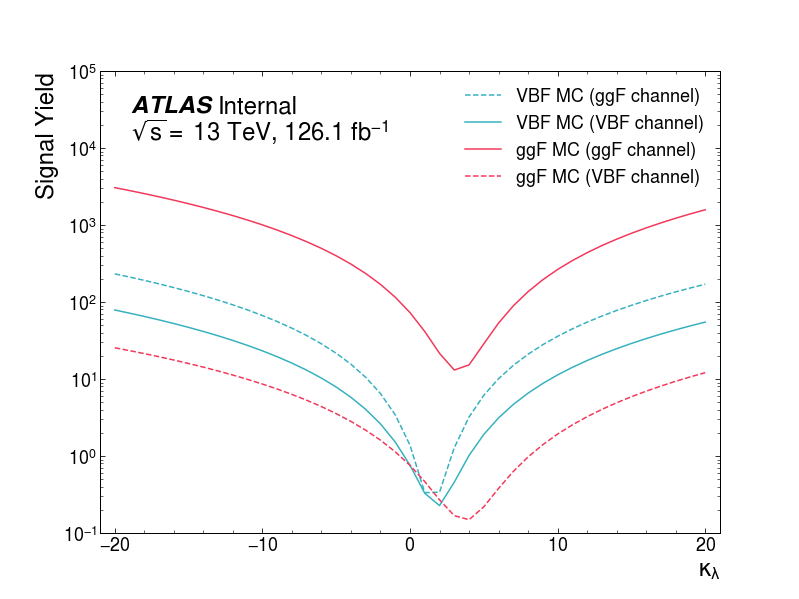
\includegraphics[width=0.48\textwidth]{figures/nr-int-note/selection/V2/signal_yield_versus_kl.png}
		\label{fig:sig_yield_kl}
	}
	\subfloat[Significance versus $\kappa_{\lambda}$]{
		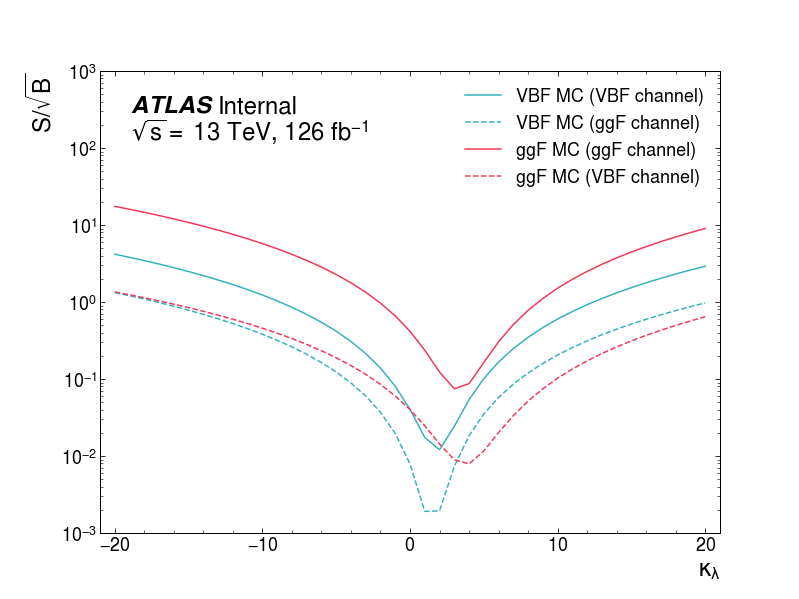
\includegraphics[width=0.48\textwidth]{figures/nr-int-note/selection/V2/s_over_sqrtb_versus_kl.png}
		\label{fig:signif_kl}
	}
	\caption{4b Signal Region yield and statistical significance of the VBF and ggF Monte Carlo simulation in the VBF and ggF SRs versus $\kappa_{\lambda}$.
	In the legend, "channel" means SR.
	}
	\label{fig:syield_signif_kl}
\end{figure}

\begin{figure}[h]
	\centering
	\subfloat[Signal yield versus $\kappa_{2V}$]{
		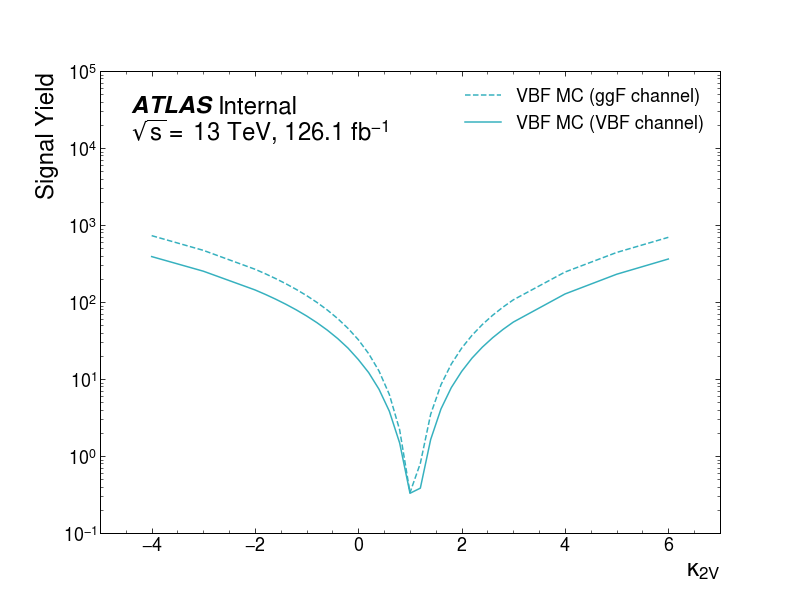
\includegraphics[width=0.48\textwidth]{figures/nr-int-note/selection/V2/signal_yield_versus_k2v.png}
		\label{fig:sig_yield_k2v}
	}
	\subfloat[Significance versus $\kappa_{2V}$]{
		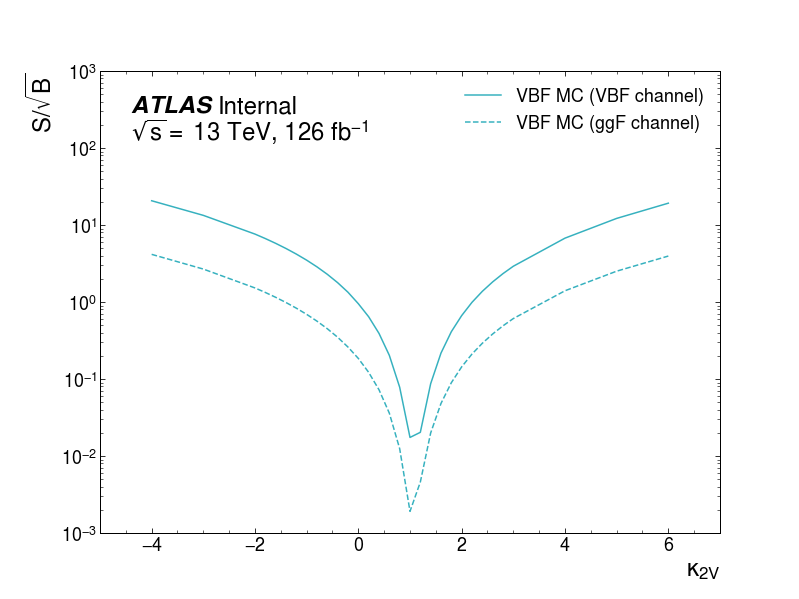
\includegraphics[width=0.48\textwidth]{figures/nr-int-note/selection/V2/s_over_sqrtb_versus_k2v.png}
		\label{fig:signif_k2v}
	}
	\caption{4b Signal Region yield and statistical significance of the VBF Monte Carlo simulation in the VBF and ggF SRs versus $\kappa_{2V}$.
	In the legend, "channel" means SR.
	}
	\label{fig:syield_signif_k2v}
\end{figure}

 \Fig{\ref{fig:accXeff}} shows the corresponding acceptance times efficiency in 1d as a function of the \kl and \kvv variations. 
Then \Fig{\ref{fig:eff-2d}} shows the corresponding acceptance times efficiency in 2d as a function of the \kl and \kvv variations. 

\begin{figure}[h]
	\centering
	\subfloat[Acceptance times efficiency versus \kl]{
		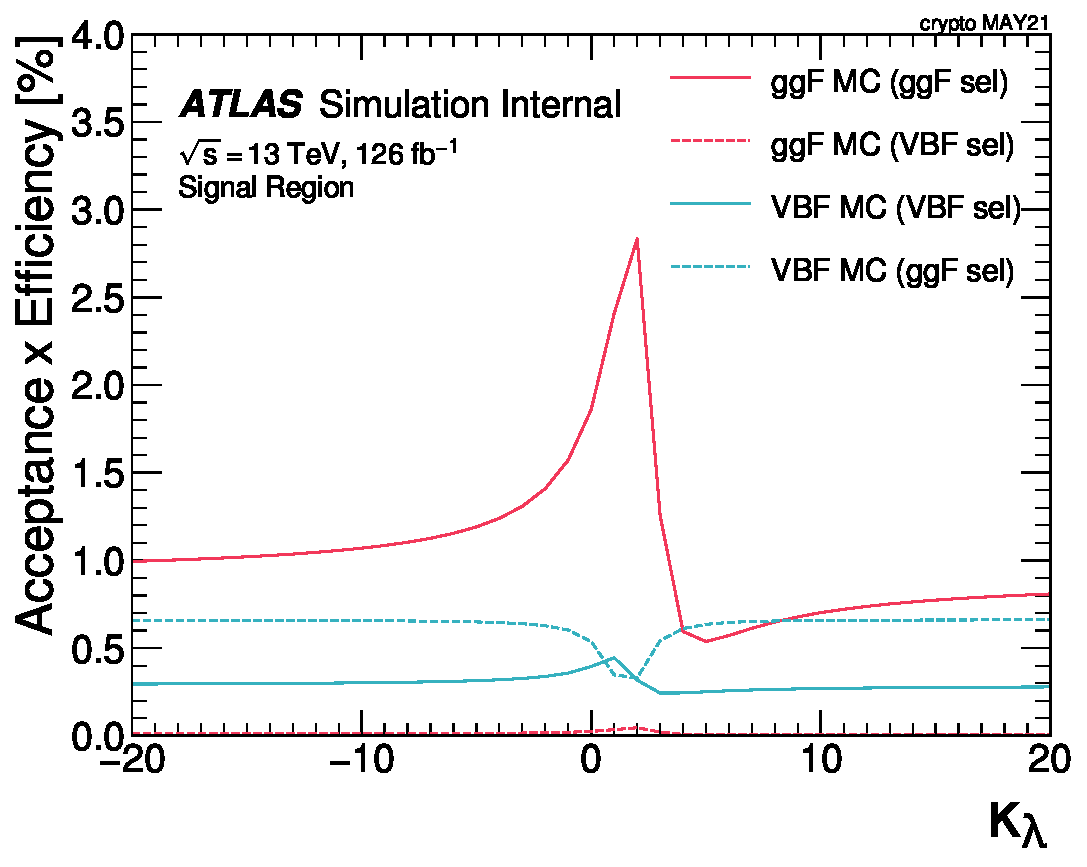
\includegraphics[width=0.48\textwidth]{figures/nr-int-note/selection/V3/accXeff_kl}
		\label{fig:accXeff_kl}
	}
	\subfloat[Acceptance times efficiency \kvv]{
		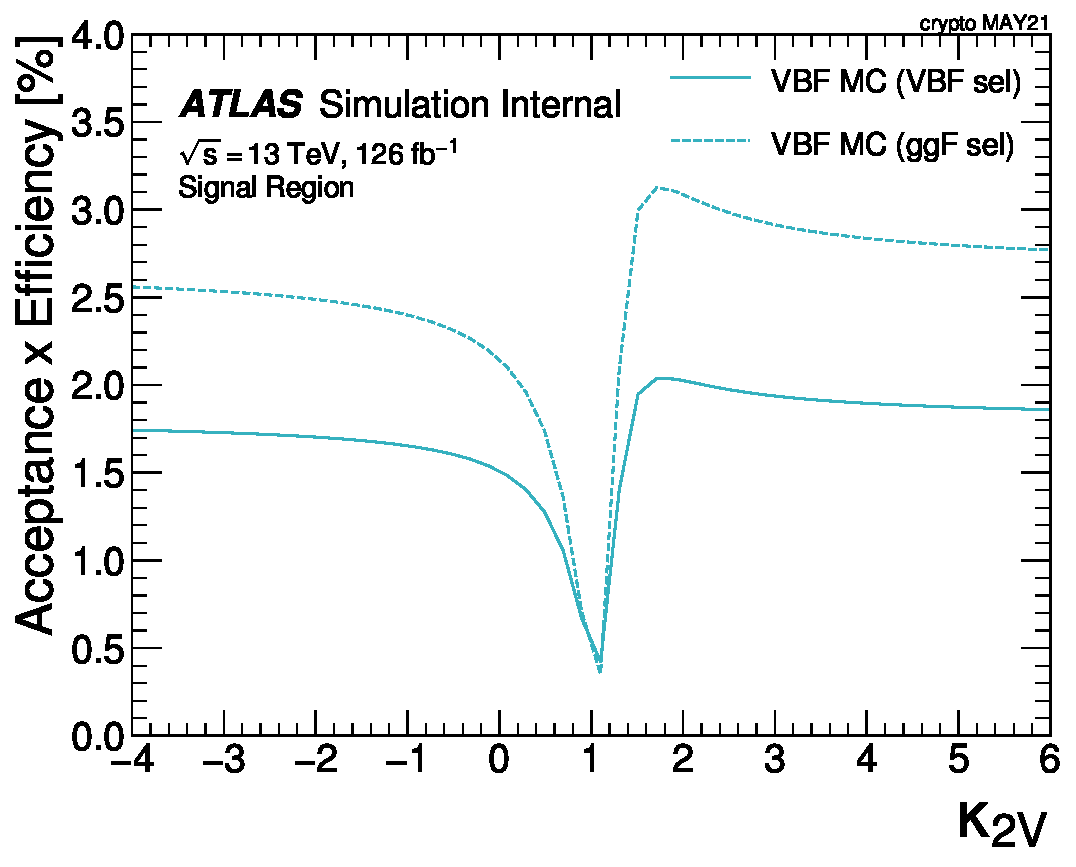
\includegraphics[width=0.48\textwidth]{figures/nr-int-note/selection/V3/accXeff_k2V}
		\label{fig:accXeff_k2V}
	}
	\caption{4b Signal Region acceptance times efficiency versus \kl and \kvv.}
	\label{fig:accXeff}
\end{figure}


\begin{figure}[h]
	\centering
	\subfloat[VBF selection]{
	    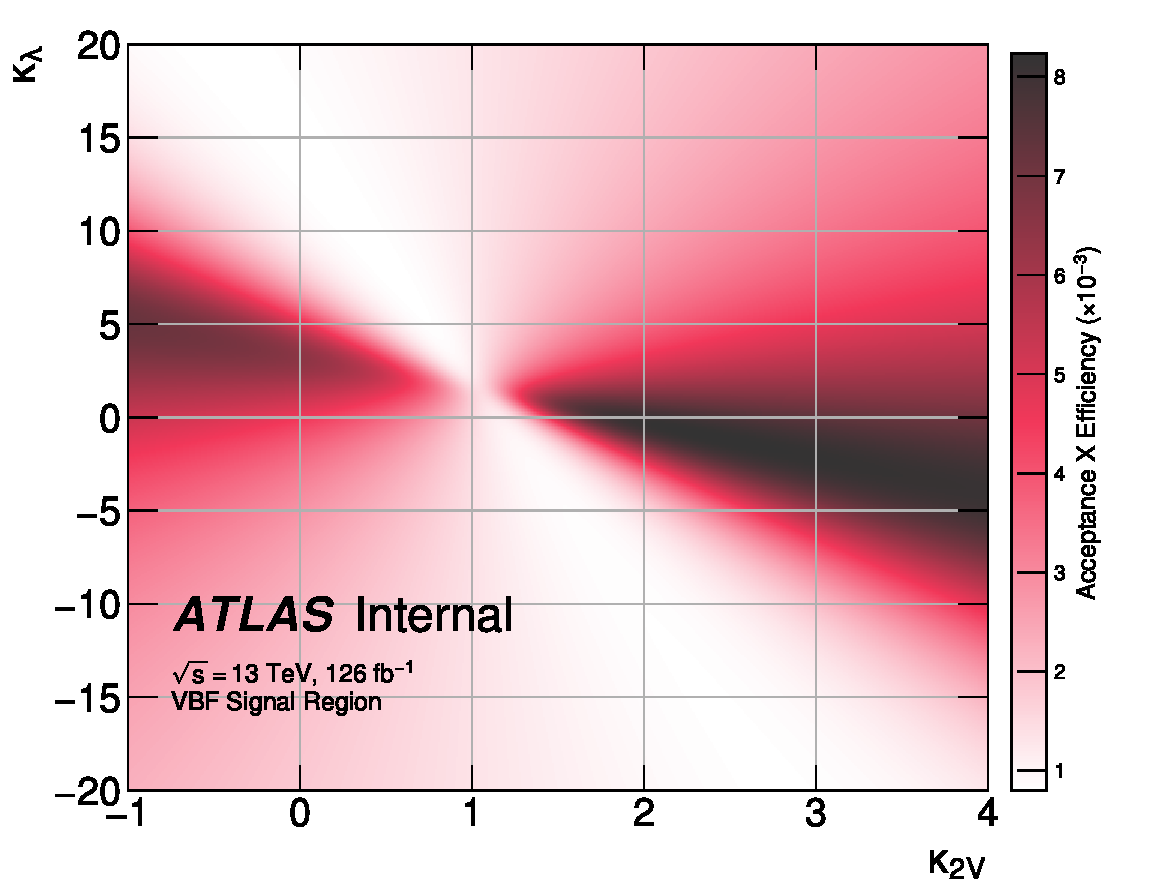
\includegraphics[width=0.7\textwidth]{figures/nr-int-note/selection/V3/VBFefficiency2D-vbf-MC-Signal-Region-all-4b}
	}
	\subfloat[ggF selection]{
	    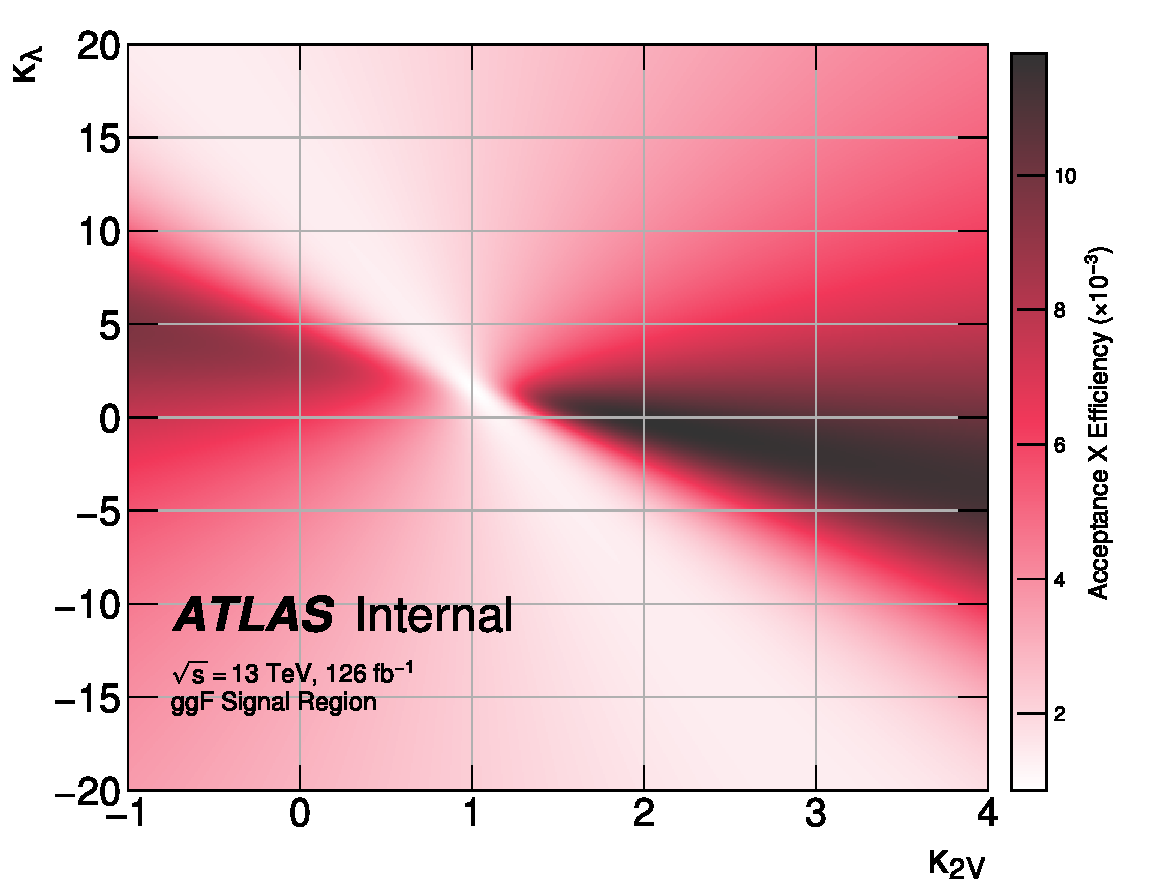
\includegraphics[width=0.7\textwidth]{figures/nr-int-note/selection/V3/VBFefficiency2D-ggf-MC-Signal-Region-all-4b}
	}
	\caption{4b Signal Region acceptance times efficiency for the VBF SM Monte Carlo simulation in the VBF or ggF selection in \kvv-\kl plane.}
	\label{fig:eff-2d}
\end{figure}

Finally, to visualize our analysis selection as we propagate through the cutflow chain, the plots for acceptance times efficiency as we propagate through the cutflow acceptance are shown in \Fig{\ref{fig:accXeff-cutflow}}. Here we show the categories driving our analysis sensitivity the ggF signal in the ggF channel and the VBF signals in the VBF channel.  In \App{\ref{app:evt-sel}}, \Fig{\ref{fig:accXeff-cutflow-app}} shows the ggF production $\kl$ cutflows in the VBF channel and the VBF production cutflows for the ggF channel.

\begin{figure}[h]
	\centering
	\subfloat[ggF MC: \kl variation]{
		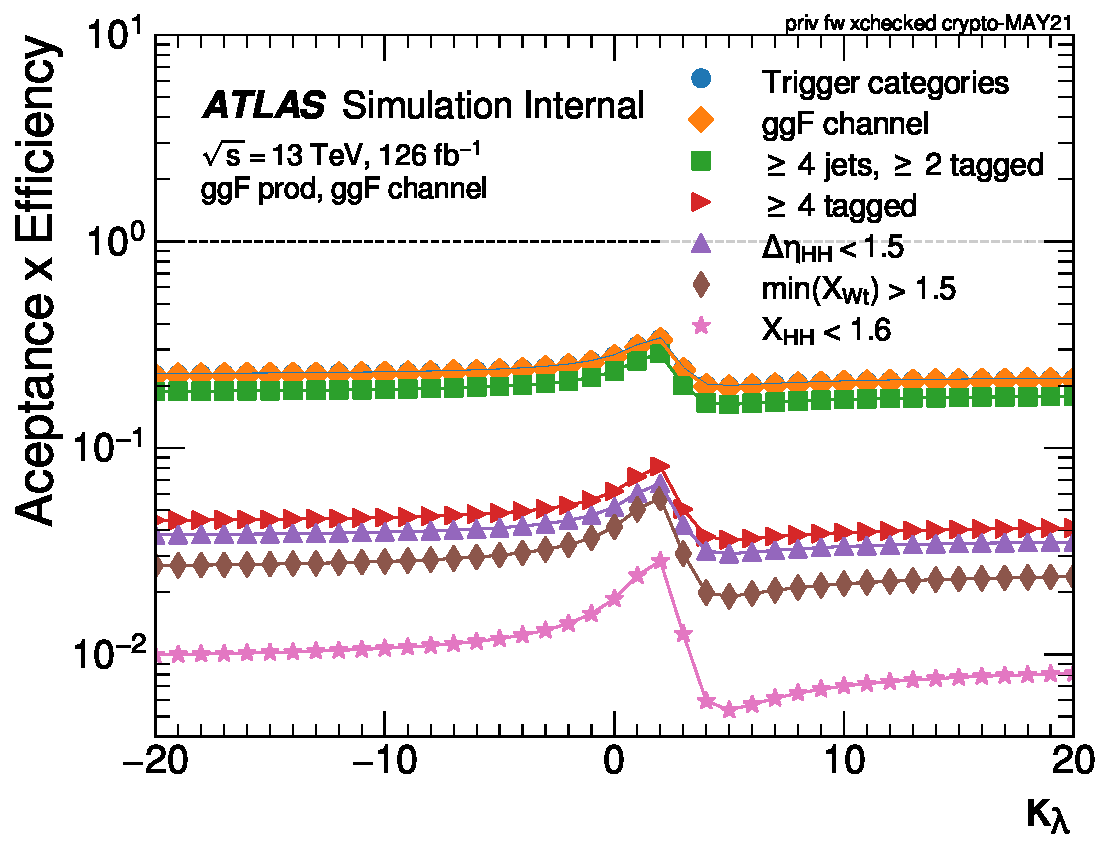
\includegraphics[width=0.48\textwidth]{figures/nr-int-note/selection/V3/acc_x_eff_ggF_kl_ggF_chan_log}
		\label{fig:accXeff_ggF_kl-ggF-sel-cutflow}
	}
	\subfloat[VBF MC: \kl variation]{
		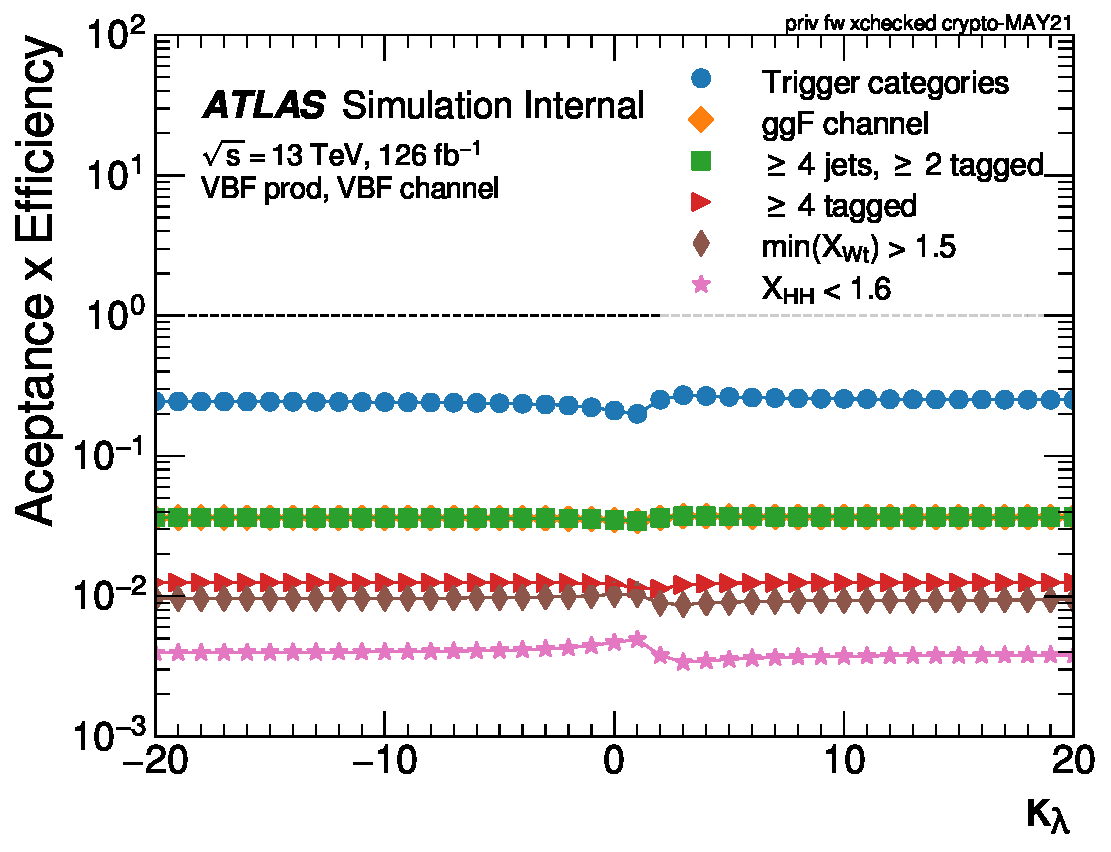
\includegraphics[width=0.48\textwidth]{figures/nr-int-note/selection/V3/acc_x_eff_VBF_kl_VBF_chan_log}
		\label{fig:accXeff_VBF_kl-VBF-sel-cutflow}
	} \\
	\subfloat[VBF MC: \kvv variation]{
		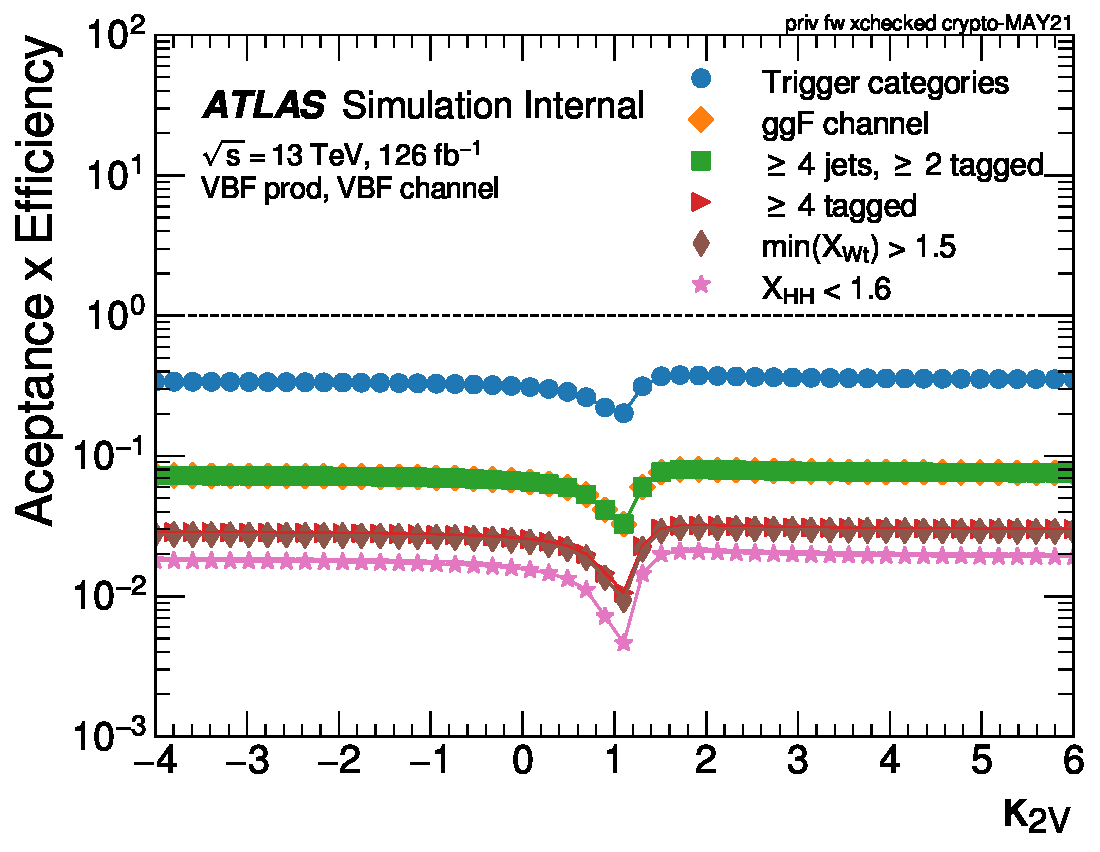
\includegraphics[width=0.48\textwidth]{figures/nr-int-note/selection/V3/acc_x_eff_VBF_k2v_VBF_chan_log}
		\label{fig:accXeff_k2V-cutflow}
	}
	\caption{4b Signal Region acceptance times efficiency.}
	\label{fig:accXeff-cutflow}
\end{figure}

